\chapter{Integrazione di Monte Carlo}\label{chapter6}
Il Rendering \`e fondato su equazioni integrali, le quali, non possiedono una forma chiusa generale, per metodi numerici come la regola del trapezio
possiedono convergenza lenta per integrali multidimensionali e discontinui, oltre a richiedere un gran numero di sample points, crescente 
esponenzialmente con la dimensionalit\`a del problema (\textit{Curse of Dimensionality}).\par
Dunque, per risolvere tali problemi, si opta ad un approccio non deterministico, Monte Carlo Integration, il quale ci permette di stimare il valore 
di un integrale $\int f(x)\mathrm{d}x$ arbitrario con il solo prerequisito di poter calcolare la funzione integranda in determinati punti.\par
Si noti che gli algoritmi di Monte Carlo, in quanto basano la scelta dei punti del dominio in cui valutare la funzione integranda casualmente, 
\textit{forniscono diversi risultati} in ogni esecuzione, dato lo stesso input, ma forniscono un risultato che \textit{statisticamente, in media, 
\`e vicino alla soluzione corretta}\footnotemark{}.
\footnotetext{Per essere pi\`u precisi, si dovrebbe affermare che il risultato fornito \textit{converge in probabilit\`a} alla soluzione}
\section{Preliminari}
Introduciamo il concetto statistico di \textit{Stimatore}
\begin{definitionS}
	Si supponga $S$ sia un parametro (di un campione o di una distribuzione) da calcolare, detto \textit{Stimando}. Uno \textit{Stimatore} 
	$\tilde{S}_n$ \`e una funzione di una collezione di variabili aleatorie $X_i$ che mappa lo spazio campionario a una \textit{Stima}. Tale Stimatore
	\`e dunque una variabile casuale del tipo
\end{definitionS}
\begin{equation}
	\tilde{S}_n = f(X_1,X_2,\ldots,X_n)
\end{equation}
La convergenza di uno Stimatore \`e qualificata a seconda di quanto "forte e stringente" tale convergenza \`e. In particolare, data una sequenza di 
variabili aleatorie $X_n$, ci sono tre modi in cui essa pu\`o convergere ad una variabile aleatoria $X$
\begin{altDescription}{chapter6:begin:convergence}
	\item[Convergenza in Distribuzione] le CDF di $X_n$, $F_{X_n}$ convergono puntualmente alla CDF di $X$, $F_X$ in tutti i punti in 
		cui essa \`e definita e continua.
		\begin{equation}
			X_n\stackrel{d}{\rightarrow}X\;\mathrm{iff}\;\lim_{n\to\infty}F_{X_n}(x)=F_X(x)
		\end{equation}
		Si noti che \`e la tipologia di convergenza pi\`u debole in quanto non restringe in alcun modo le osservazioni estratte da ciascuna delle 
		variabili aleatorie
	\item[Convergenza in Probabilit\`a] La probabilit\`a di vicinanza arbitraria tra le osservazioni di $X_n$ e $X$ cresce man mano che si prosegue
		nella sequenza
		\begin{equation}
			X_n\stackrel{p}{\rightarrow}X\;\mathrm{iff}\;\lim_{n\to\infty}\Pr(|X_n-X|\geq\varepsilon)=0\;\forall\varepsilon>0
		\end{equation}
		Si noti che ci\`o non assicura la correttezza di alcuna osservazione della sequenza, soltanto che \`e molto improbabile discostarsi di molto 
		dal valore esatto per $n$ sufficientemente grande
	\item[Convergenza Quasi Certa] Il sottoinsieme $\bar{\Omega}$ nel quale le osservazioni della sequenza si discostano dal valore vero \`e finito.
		Ci\`o vuol dire che, al limite, la convergenza \`e assicurata, con esattezza quasi certa, per via dell'esistenza di finiti valori errati nelle
		osservazioni della sequenza
		\begin{equation}
			X_n\stackrel{a.s.}{\rightarrow}X\;\mathrm{iff}\;\Pr\left(\left\{\omega\in\Omega\,:\,\lim_{n\to\infty}X_n(\omega)=X(\omega)\right\}\right)=1	
		\end{equation}
\end{altDescription}
Maggiore \`e il "grado di convergenza", e maggiore \`e la frequenza in cui lo stimatore ci restituisce un risultato quasi esatto. Dunque si dice
\textit{Debolmente Consistente} uno Stimatore che converge in probabilit\`a allo stimando, e \textit{Fortemente Consistente} uno Stimatore che 
converge quasi certamente allo stimando.\par
Tale parametro pu\`o essere stimato con lo stimatore \textit{Media Campionaria}, il quale \`e definito come 
\begin{equation}
	\tilde{E}_n[X]=\frac{1}{n}\sum_{i=1}^nx_i
\end{equation}
dove $\{x_1,\ldots,x_n\}$ campione estratto casualmente da un insieme di $n$ variabili aleatorie indipendenti e identicamente distribuite (i.i.d.) 
$X_i$.
Tale stima pu\`o essere incrementalmente raffinata come 
\begin{equation}
	\tilde{E}_i[X]=\frac{(i-1)\tilde{E}_{i-1}[X]+x_i}{i}
\end{equation}
Si dimostra, rispettivamente, tramite la WLLN (Legge dei grandi numeri debole) che lo stimatore media campionaria \`e debolmente consistente, e tramite
la SLLN (Legge dei grandi numeri forte) che lo stimatore \textit{media campionaria \`e fortemente consistente}. Ci\`o, assieme al fatto che 
tale stimatore altro non fa che stimare un integrale, rende la media campionaria un ottimo candidato per formulare lo stimatore di Monte Carlo.\par
\section{Monte Carlo Integration}
Si ricordi che la aspettazione di una variabile aleatoria $X$, la cui PDF $p_X$ definita in un dominio $D$ \`e pari a 
\mbox{$E[X]=\int_Dxp_X(x)\mathrm{d}x$}, per la quale vale la seguente propriet\`a: sia $y=f(x)$, allora
\begin{equation*}
	E[f(X)]=\int_{\Omega_y}yp_Y(y)\mathrm{d}y=\int_{\Omega_x}f(x)p_y(f(x))\left|\det(J_f(x))\right|\mathrm{d}x=\int_{\Omega_x}f(x)p_X(x)\mathrm{d}x
\end{equation*}
\`E possibile ricavare uno stimatore per l'integrale di una funzione integranda arbitraria $f(x)$
\begin{equation}
	E\left[\frac{f(X)}{p_X(X)}\right]=\int_{\mathcal{D}}\frac{f(x)}{p_X(x)}p_X(x)\mathrm{d}x=\int_{\mathcal{D}}f(x)\mathrm{d}x
\end{equation}
Assumendo densit\`a di probabilit\`a uniforme nel dominio $\mathcal{D}$, si ottiene
\begin{equation}
	\norm{\mathcal{D}}E[f(X)]=\norm{\mathcal{D}}\int_{\mathcal{D}}f(x)p_X(x)\mathrm{d}x=\int_{\mathcal{D}}f(x)\mathrm{d}x
\end{equation}
Sostituendo l'aspettazione con la media campionaria, otteniamo uno stimatore \textit{unbiased}\footnotemark{} per l'integrale
\begin{equation}\label{chapter6:MC:crudeEstimator}
	\tilde{F}_n=\norm{\mathcal{D}}\tilde{E}_n[f(X)]=\frac{\norm{\mathcal{D}}}{n}\sum_{i=1}^nf(X_i)
\end{equation}
\footnotetext{vedi sezioni seguenti}
\begin{figure}[tb]
	\centering
	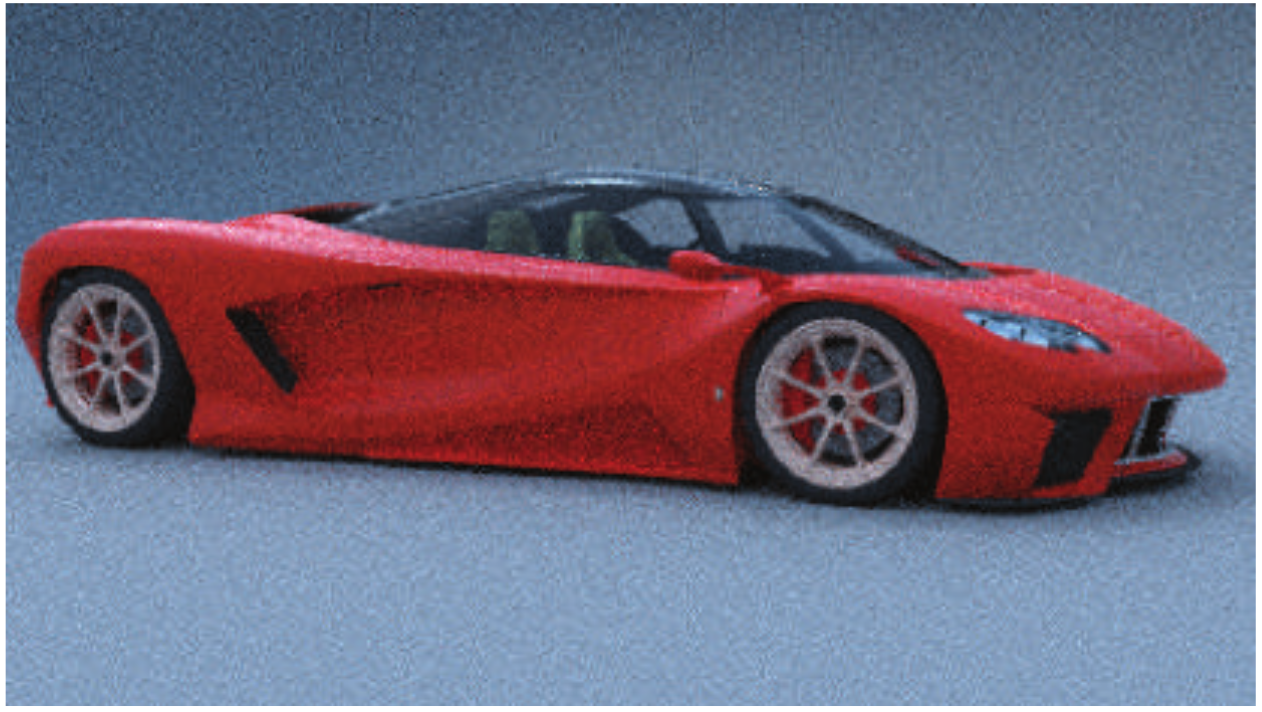
\includegraphics[width=0.7\linewidth]{../assets/chapter6_MC_variance.png}
	\caption{Illustrazione della varianza in una immagine renderizzata. Immagine da \cite{pharr}}
	\label{chapter6:MC:variance}
\end{figure}
Rilasseremo in seguito, all'introduzione di Importance Sampling, l'assunzione di campionamento con PDF uniforme, giungendo a
\begin{equation}\label{chapter6:MC:importanceEstimator}
	\tilde{F}_n=\norm{\mathcal{D}}\tilde{E}_n[f(X)]=\frac{1}{n}\sum_{i=1}^n\frac{f(X_i)}{p(X_i)}
\end{equation}
Una misura di accuratezza di tale stimatore \`e la sua varianza, la quale si traduce, nell'immagine renderizzata, in variazioni brusche tra pixel 
adiacenti, come mostrato in Figura \ref{chapter6:MC:variance}. Tale varianza\footnotemark{}, per lo stimatore in 
Equazione \ref{chapter6:MC:crudeEstimator}
\begin{align}\label{chapter6:MC:crudeVariance}
	V[\tilde{F}_n]&=V\left[\norm{\mathcal{D}}\tilde{E}_n[f(X)]\right]=\norm{\mathcal{D}}^2V\left[\tilde{E}_n[f(X)]\right]%
	=\frac{\norm{\mathcal{D}}^2}{n}V[f(X)] \\
	&=\frac{\norm{\mathcal{D}}^2}{n}\frac{1}{\norm{\mathcal{D}}}\int_{\mathcal{D}}(f(x)-\bar{f})^2\mathrm{d}x=
	\frac{\norm{\mathcal{D}}}{n}\int_{\mathcal{D}}f(x)^2\mathrm{d}x-\bar{f}^2 \nonumber
\end{align}
Da cui la deviazione standard, la quale rappresenta l'errore dello stimatore di monte carlo, \`e pari a
\begin{equation}
	\sigma[\tilde{F}_n]=\sqrt{V[\tilde{F}_n]}=\sqrt{\frac{\norm{\mathcal{D}}^2}{n}V[f(X)]}=\frac{\norm{\mathcal{D}}}{n^{\frac{1}{2}}}\sigma[f(X)]
\end{equation}
Essa diminuisce come \mbox{$\mathcal{O}\left(n^{-\frac{1}{2}}\right)$}, Il che dimostra che l'\textit{ordine di convergenza} dello stimatore \`e 
$1/2$. Esso \`e chiamato "diminishing return" dal fatto che 
per abbattere l'errore atteso di un fattore $1/n$ bisogna campionare $n^2$ volte la funzione in esame. Si noti che tecniche di quadratura 
convergono pi\`u velocemente per integrali 1D, ma appena si passa a integrali multidimensionali il loro costo e convergenza peggiorano 
considerevolmente, mentre la accuratezza di Monte Carlo non dipende dalla dimensionalit\`a, rendendolo l'unica alternativa.
\footnotetext{Ricordiamo che $V[aX+b]=a^2V[X]$ e che, se le variabili $\left\{X_i\right\}_{i=1}^n$ sono incorrelate, 
	\mbox{$V\left[\tilde{E}_n[f(X)]\right]=V[X]/n$}}
Altre caratteristiche dello stimatore sono \textit{efficienza}, \textit{bias}, \textit{mse}
\begin{altDescription}{qualities}
	\item[Bias] Differenza tra aspettazione dello stimatore e lo stimando
		\begin{equation}
			\beta = E[\tilde{F}_n(X)]-\int_{\mathcal{D}}f(x)\mathrm{d}x
		\end{equation}
		Nonostante sembrino sconvenienti, in quanto non tendono al valore desiderato, possono comunque risultare vantaggiosi nel caso si desideri uno
		stimatore con varianza minore. Per esempio, lo stimatore biased per la aspettazione
		\begin{equation}
			\frac{1}{2}\max\{X_1,X_2,\ldots,X_n\}
		\end{equation}
		ha deviazione standard che segue \mbox{$\mathcal{O}\left(n^{-1}\right)$}
	\item[Efficienza] Parametro che permette di stimare la bont\`a di uno stimatore in relazione alla varianza ottenuta $V[X]$ e al suo running time
		$T[X]$, pari a 
		\begin{equation}\label{chapter6:MC:efficiency}
			\epsilon[\tilde{F}_n]=\frac{1}{V[\tilde{F}_n]T[\tilde{F}_n]}
		\end{equation}
	\item[MSE] Errore quadratico medio, strettamente collegato alla varianza, in quanto \`e definito come l'aspettezione del quadrato della 
		differenza tra uno stimatore ed il valore vero
		\begin{equation}
			MSE[\tilde{F}_n]=E\left[\left(\tilde{F}_n-\int_{\mathcal{D}}f(x)\mathrm{d}x\right)^2\right]=V[\tilde{F}_n]+\beta^2
		\end{equation}
		Tale metrica risulta utile quando si \`e a conoscenza di una previa stima, magari con un numero elevato di campioni, di un integrale $F$,
		per la quale possiamo applicare lo stimatore media campionaria per calcolarne il suo valore approssimato.
\end{altDescription}
\section{Esempio: Risoluzione di Integrali Semplici}\label{chapter6:MCExample}
\begin{figure}[t]
	\centering
	\begin{subfigure}[t]{0.45\linewidth}
		\begin{scaletikzpicturetowidth}{\linewidth}\begin{tikzpicture}[scale=\tikzscale]
			\begin{axis} [
				axis lines = left,
				ylabel=$f(x)$,
				xlabel=$x$,
				ymin=0, ymax=4,
				xmin=0, xmax=11,
				declare function={
					s(\x)=sqrt(((pi^2)/10)*\x);
					func(\x)=sin(s(\x)*180/pi)*e^s(\x)/s(\x);
				},
			]
				\addplot[color=black, domain=0.001:11, domain y=0:4, samples=50,]{func(x)};
			\end{axis}
		\end{tikzpicture}\end{scaletikzpicturetowidth}
		\caption{Funzione specificata in Equazione \ref{chapter6:MCExample:function}}
	\end{subfigure}
	\begin{subfigure}[t]{0.45\linewidth}
		\begin{scaletikzpicturetowidth}{\linewidth}\begin{tikzpicture}[scale=\tikzscale]
			\begin{axis} [
				axis lines = left,
				xlabel=nSamples,
				ylabel=$\tilde{F}_n-F$,
				ymax=2, ymin=-2,
			]
				\addplot [black,] table[ignore chars={(,)},col sep=comma] {../assets/chapter6_error_data.dat};
			\end{axis}
		\end{tikzpicture}\end{scaletikzpicturetowidth}
		\caption{Funzione Errore}
		\label{chapter6:MCExample:1Dfunction:error}
	\end{subfigure}
	\caption{Grafico della funzione nell'Esempio di Sezione \ref{chapter6:MCExample}, con errore della stima ottenuta da Equazione 
		\ref{chapter6:MC:crudeEstimator}}
	\label{chapter6:MCExample:1Dfunction}
\end{figure}
\begin{figure}[tb!]
	\centering
	\begin{subfigure}[t]{0.45\linewidth}
		\begin{scaletikzpicturetowidth}{\linewidth}\begin{tikzpicture}[scale=\tikzscale]
			\begin{axis} [
				axis lines = left,
				xlabel=nSamples,
				ylabel=$\tilde{F}_n^{\beta}-F$,
				ymin=-2, ymax=0,
			]
				\addplot [black,] table[ignore chars={(,)},col sep=comma] {../assets/chapter6_biased_estimator_error_data.dat};
			\end{axis}
		\end{tikzpicture}\end{scaletikzpicturetowidth}
		\caption{Funzione errore derivata dall'uso dello stimatore biased $\tfrac{1}{2}\operatorname{max}\{f(X_1),\ldots\}$. 
			Si osserva come la varianza sia visibilmente diminuita, a costo della convergenza al valore corretto.}
		\label{chapter6:MCExample:1Dfunction:bias}
	\end{subfigure}
	\begin{subfigure}[t]{0.45\linewidth}
		\begin{scaletikzpicturetowidth}{\linewidth}\begin{tikzpicture}[scale=\tikzscale]
			\begin{axis} [
				axis lines = left,
				xlabel=nSamples,
				ylabel={$MSE\left[\tilde{F}_n\right]$},
				ymax=5, ymin=0,
			]
				\addplot [black,] table[ignore chars={(,)},col sep=comma] {../assets/chapter6_mse_data.dat};
			\end{axis}
		\end{tikzpicture}\end{scaletikzpicturetowidth}
		\caption{$MSE$ dello stimatore unbiased}
		\label{chapter6:MCExample:1Dfunction:mse}
	\end{subfigure}
	\begin{subfigure}[t]{0.45\linewidth}
		\begin{scaletikzpicturetowidth}{\linewidth}\begin{tikzpicture}[scale=\tikzscale]
			\begin{axis} [
				axis lines = left,
				xlabel=nSamples,
				ylabel={$\epsilon\left[\tilde{F}_n\right]$},
				ymax=5, ymin=0,
			]
				\addplot [black,] table[ignore chars={(,)},col sep=comma] {../assets/chapter6_efficiency.dat};
			\end{axis}
		\end{tikzpicture}\end{scaletikzpicturetowidth}
		\caption{Funzione efficienza $\epsilon\left[\tilde{F}_n\right]=\tfrac{1}{V[\tilde{F}_n]T[\tilde{F}_n]}$ dello stimatore unbiased. 
			Si noti come esso presenta varie fluttuazioni, derivanti dalle condizioni continuamente variabili del calcolatore.}
		\label{chapter6:MCExample:1Dfunction:efficiency}
	\end{subfigure}
	\caption{Ulteriori risultati dell'Esempio presentato in Sezione \ref{chapter6:MCExample}}
	\label{chapter6:MC:plots}
\end{figure}
Al fine di rendere chiara l'applicazione della Equazione \ref{chapter6:MC:crudeEstimator} al calcolo degli integrali, applichiamo il metodo di 
Monte Carlo all'integrale definito in $[0,10]$ della seguente funzione:
\begin{equation}\label{chapter6:MCExample:function}
	f(x)=\frac{\sin\left(\sqrt{\frac{\pi^{2}}{10}x}\right)}{\sqrt{\frac{\pi^{2}}{10}x}}e^{\sqrt{\frac{\pi^{2}}{10}x}}
\end{equation}
per la quale \`e possibile giungere alla soluzione analitica
\begin{equation}
	\hat{f}(x)=
		\frac{10\left(\sin\left(\pi\sqrt{\frac{x}{10}}\right)−\cos\left(\pi\sqrt{\frac{x}{10}}\right)\right)e^{\pi\sqrt{\frac{x}{10}}}}{\pi^2} + C
\end{equation}
Per cui il valore di tale integrale \`e noto e pari a 
\begin{equation}
	F = \int_0^{10}f(x)\mathrm{d}x = \hat{f}(10) - \hat{f}(0) = \frac{10e^\pi+10}{\pi^2}\approx 24.45963551499059
\end{equation}
Al fine di poter stimare numericamente tale integrale, \`e stata applicata Equazione \ref{chapter6:MC:crudeEstimator}, dove i campioni $x_i$ sono stati
estratti con distribuzione uniforme nel dominio $[0,10]$, la cui generazione \`e stata implementata mediante la libreria \texttt{numpy}. In particolare,
dei generatori supportati, \`e stato utilizzato un Generatore Congruenziale Permutato
\footnote{Brevemente introdotti in Appendice \ref{appendixC}, per pi\`u informazioni si rimanda a 
\href{https://en.wikipedia.org/wiki/Permuted\_congruential\_generator}{https://en.wikipedia.org/wiki/Permuted\_congruential\_generator}}
I risultati ottenuti dalla simulazione di Monte Carlo con codice mostrato in Appendice \ref{appendixD:MC} sono mostrati in Figura 
\ref{chapter6:MCExample:1Dfunction}\subref{chapter6:MCExample:1Dfunction:error} e Figura \ref{chapter6:MC:plots}
\section{Schemi di Campionamento}
Supponendo si abbia a disposizione un algoritmo per estrarre un numero casuale uniformemente distribuito nell'intervallo $[0,1]$ 
(Appendice \ref{appendixC:RNG}) oppure un algoritmo che permetta di estrarre numeri quasirandom da una sequenza con low discrepancy 
(Sezione \ref{chapter5:sampling:QuasiMonteCarlo}),
analizziamo metodi per poter campionare samples da una distribuzione arbitraria, come quelle analizzate in Capitolo \ref{chapter3}.\par
Le tre tecniche che citiamo a tal scopo sono \textit{Inverse Transform Sampling}, \textit{Acceptance-Rejection Sampling}, 
\textit{Metropolis Hastings Sampling}
\subsection{Inverse Transform Sampling}\label{chapter6:sampling:inverseTransformSection}
\begin{figure}[tb]
	\centering
	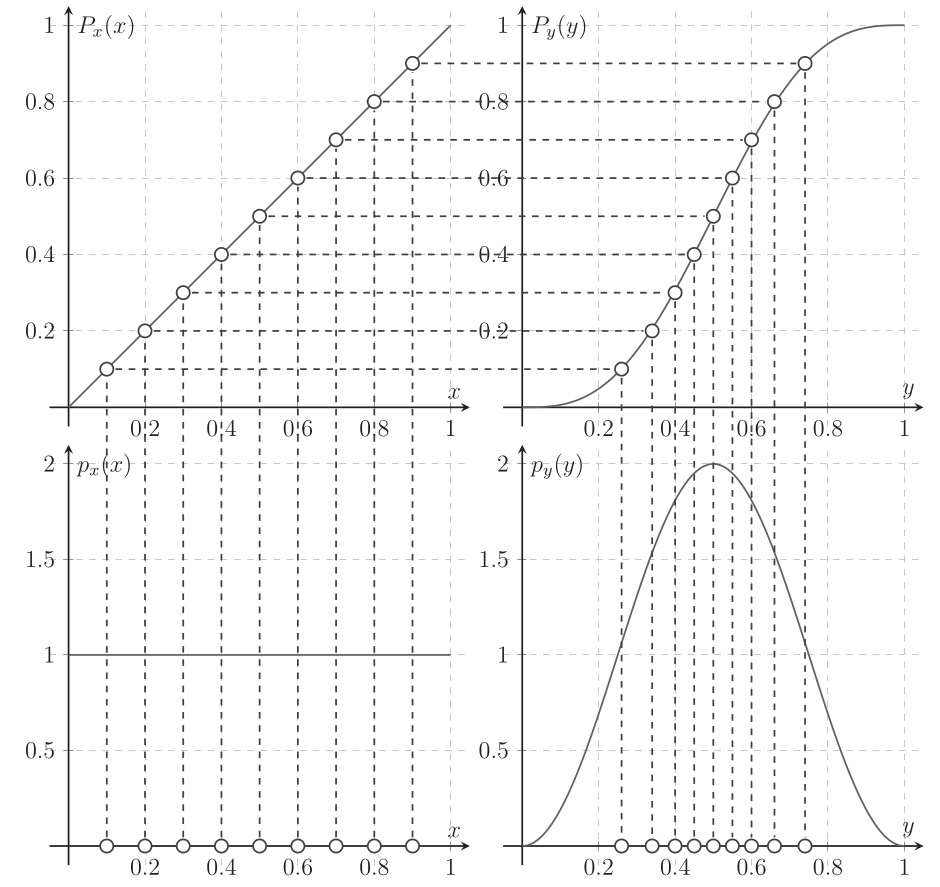
\includegraphics[width=0.9\linewidth]{../assets/chapter6_sampling_inverse_transform_sampling.png}
	\caption{Illustrazione della tasformazione di samples tra due PDFs (riga inferiore) usando le loro CDFs (riga superiore). Immagine da 
		\cite{pegoraro}}
	\label{chapter6:sampling:inverseTransform}
\end{figure}
Date due variabili casuali $X$ e $Y$, di CDFs\footnotemark{} $P_x$ e $P_y$, gi\`a calcolate analiticamente, e la possibilit\`a di campionare $X$ ed 
ottenere 
\footnotetext{Questo metodo funziona anche nel discreto, sostituendo PDF con PMF e integrali con somme}
osservazioni $x$, possiamo trasformare tali campioni in campioni $y$ secondo la seguente procedura:\par
\begin{itemize}[topsep=0pt,noitemsep]
	\item Calcolare la \textit{funzione quantile} della variabile aleatoria $Y$, $P_y^{-1}$
	\item La variabile aleatoria $Y$ \`e dunque posta a $P_y^{-1}(P_x(X))$
\end{itemize}
Dove la funzione quantile altro non \`e che una funzione di distribuzione inversa generalizzata, la quale rende possibile invertire CDFs con intervalli
costanti
\begin{equation}
	P_y^{-1}(p)=\inf\left\{y\in\mathbb{R}^d\,:\,P_y(y)\geq p\right\},\;p\in[0,1]
\end{equation}
Il procedimento \`e illustrato in Figura \ref{chapter6:sampling:inverseTransform}.\par
Nel caso di una distribuzione multivariata, l'inverse transform sampling \`e un processo iterativo nel quale, scelta una prima dimensione in cui
campionare, si calcola la sua CDF marginale per poi invertirla e trasformare la prima dimensione del campione iniziale. In seguito, tutte le 
altre dimensioni sono calcolate mantenendo fisse le dimensioni gi\`a campionate mediante il calcolo di CDFs condizionali della dimensione corrente, 
dato il valore fissato di tutte le dimensioni gi\`a campionate, e la loro inversione permette di portare a termine la computazione.\par
Ad esempio, data una PDF multivariata bidimensionale $p(x,y)$, una coordinata casuale $x_i$ pu\`o essere campionata applicando la procedura di 
inverse transform sampling alla sua PDF marginale $p_x(x)=\int_{\Omega_y}p(x,y)\mathrm{d}y$, mentre una coordinata casuale $y_i$ pu\`o essere 
campionata applicando la procedura di inverse transform sampling alla PDF condizionale $p_{y|x}(y|x_i)=p(x_i,y) / p_x(x_i)$.\par
Nel caso in cui la PDF congiunta risulta separabile, cio\`e le variabili sono indipendenti 
\mbox{$\int\int p(x,y)\mathrm{d}x\mathrm{d}y=\int p_x(x)\mathrm{d}x\int p_y(y)\mathrm{d}y$} allora siamo in grado di applicare inverse transform 
sampling a ciascuna coordinata utilizzando le rispettive PDFs marginali.
\subsection{Acceptance-Rejection Method}
\begin{figure}[tb]
	\centering
	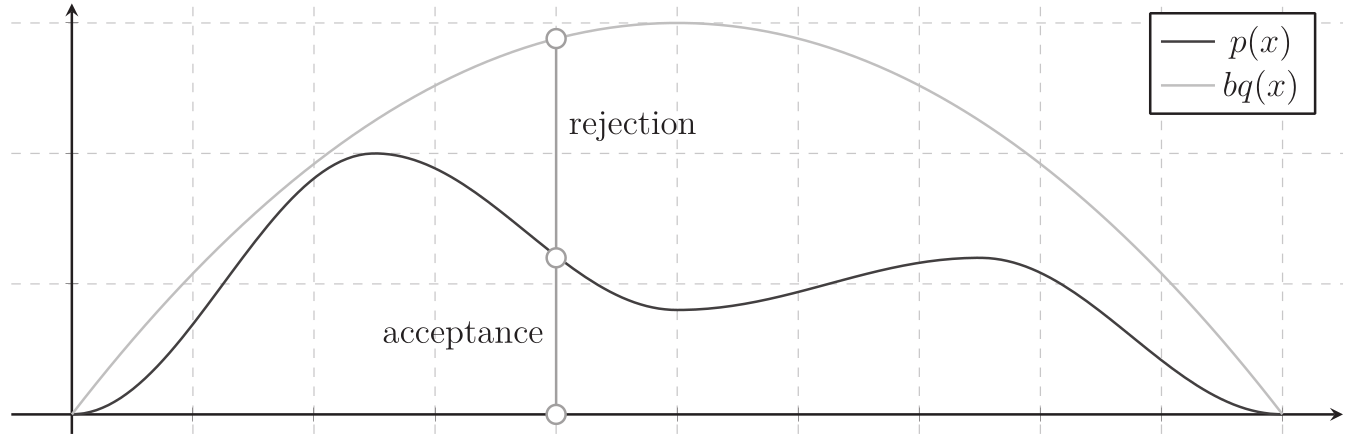
\includegraphics[width=0.8\linewidth]{../assets/chapter6_sampling_acceptance_rejection.png}
	\caption{Illustrazione del rejection sampling. Immagine da \cite{pegoraro}}
	\label{chapter6:sampling:rejectionSampling}
\end{figure}
Alcune funzioni, una volta normalizzate\footnotemark{}, possiedono CDFs non invertibili o non calcolabili. Il metodo 
\textit{Acceptance-Rejection Sampling} permette di campionare samples secondo una data PDF $p(x)$ supponendo di avere la possibilit\`a di campionare, 
mediante altri metodi, una PDF $q(x)$, tale che esista un upper bound $b>p(x)/q(x)$, $\forall x\in\Omega$ cio\`e
\begin{equation}
	0\leq\frac{p(x)}{bq(x)}\leq 1
\end{equation}
\footnotetext{Come spiegato in seguito, una tecnica che pu\`o ridurre la varianza nei metodi di Monte Carlo, \textit{Importance Sampling}, consiste 
	nel campionare punti in cui valutare la funzione integranda con probabilit\`a proporzionale al valore assunto dalla funzione stessa, dunque spiegata
	la necessit\`a di ricavare PDFs da funzioni arbitrarie}
L'algoritmo consiste nel
\begin{itemize}[topsep=0pt,noitemsep]
	\item Estrarre un campione $x_i$ dalla variabile aleatoria $X$, distribuito secondo la PDF $q(x)$
	\item Generare un numero casuale $\xi\sim\mathcal{U}(0,1)$
	\item Se $\xi bq(x_i)\leq p(x_i)$, allora il campione $x_i$ \`e accettato come realizzazione della PDF target $p(x)$, ed \`e rifiutato in caso
		contrario
\end{itemize}
Dato un campione $x$, la \textit{acceptance probability} \`e data da
\begin{equation}
	\Pr\left(\xi\leq\frac{p(x)}{bq(x)}\right)=\int_0^{\frac{p(x)}{bq(x)}}\mathrm{d}x^\prime=\frac{p(x)}{bq(x)}
\end{equation}
La cui aspettazione rappresenta la proporzione di campioni accettati
\begin{equation}
	E\left[\frac{p(X)}{bq(X)}\right]=\int_\Omega\frac{p(x)}{bq(x)}q(x)\mathrm{d}x=\frac{1}{b}\int_\Omega p(x)\mathrm{d}x=\frac{1}{b}
\end{equation}
\begin{figure}[tb]
	\centering
	\begin{subfigure}{0.45\linewidth}
		\begin{scaletikzpicturetowidth}{\linewidth}\begin{tikzpicture}[scale=\tikzscale]
			\begin{axis} [
				colormap/cool,
				declare function={
					func(\x,\y)=(\x^2+\y^2<=1 && \x>=0 && \y>=0) * 4/(pi);
				},
			]
				\addplot3[mesh, samples=20, domain=-0.5:1.5] {func(x,y)};
			\end{axis}
		\end{tikzpicture}\end{scaletikzpicturetowidth}
		\caption{pdf target $q(x,y)$}
	\end{subfigure}
	\begin{subfigure}{0.45\linewidth}
		\begin{scaletikzpicturetowidth}{\linewidth}\begin{tikzpicture}[scale=\tikzscale]
			\begin{axis} [
				colormap/hot,
				declare function={
					quad(\x,\y)=(0<=\x<=1 && 0<=\y<=1);
				},
			]
				\addplot3[mesh, samples=20, domain=-0.5:1.5] {quad(x,y)};
			\end{axis}
		\end{tikzpicture}\end{scaletikzpicturetowidth}
		\caption{PDF strumentale $p(x,y)$}
	\end{subfigure}
	\caption{Illustrazione delle due PDF coinvolte nell'esempio proposto per Rejection rampling}
\end{figure}
in media, dunque, $b$ campioni sono estratti in media prima di accettarne uno. Ci\`o nonostante, Rejection-Sampling pu\`o non essere efficace nel 
campionamento di distribuzioni altamente concentrate in una piccola regione del loro dominio. Inoltre, man mano che la dimensionalit\`a del problema
aumenta, il volume "in eccesso" della distribuzione strumentale aumenta, rendendo il metodo soggetto alla curse of dimensionality.\par
Per \textit{Curse of Dimensionality} si riferisce all'insieme di fenomeni che penalizzano o rallentano determinati algoritmi numerici, i quali 
diventano pi\`u evidenti man mano che la dimensionalit\`a aumenta. Nel caso del campionamento, tale problema deriva dall'aumento esponenziale del 
volume all'aggiunta di una dimensione extra in uno spazio campionario.\par
Come esempio di applicazione, si consideri il campionamento con distribuzione uniforme di un dominio pari ad un quarto di disco unitario, 
utilizzando come proposal distribution una distribuzione uniforme definita in un quadrato unitario\footnotemark{}.\par
La PDF target \`e dunque 
\begin{equation}
	q(x,y) = \left\{\begin{aligned}
		&\frac{4}{\pi}\;&\mathrm{se}\;x^2+y^2\leq1\text{ e }x,y\geq0\\
		&0 &\mathrm{altrimenti}
	\end{aligned}\right.
\end{equation}
con proposed distribution 
\begin{equation}
	p(x,y) = \left\{\begin{aligned}
		&1\;&\mathrm{se}\;(x,y)\in[0,1]^2\\
		&0 &\mathrm{altrimenti}
	\end{aligned}\right.
\end{equation}
da cui si evince che $b\geq4/\pi$, il che fa in modo che un campione sia accettato dopo aver generato $\approx1.27$ samples. Il codice Python che 
implementa tale procedura \`e in Appendice \ref{appendixD:rejectionSampling}
\label{appendixD:rejectionSampling}.
\footnotetext{\`E interessante notare come, riformulando tale procedura come mostrato in \textrm{alt\_rejection\_sampling}, si possa stimare il valore 
di $\pi$}
\subsection{Metriopolis-Hastings Sampling}
Piuttosto che generare campioni in maniera indipendente, costruiamo una \textit{Markov Chain} co\-stituente un Randow Walk nello spazio campionario,
la cui distribuzione, al limite, converge alla distribuzione desiderata, detta \textit{distribuzione stazionaria} o distribuzione all'equilibrio. I 
vantaggi rispetto agli altri metodi qui presentati sono
\begin{itemize}[topsep=0pt,noitemsep]
	\item Ogni iterazione produce un campione
	\item Non richiede la normalizzazione della funzione target $f(x)$. Vedi Equazione \ref{chapter6:metropolis:acceptance}
	\item Non richiede una CDF calcolabile ed invertibile
\end{itemize}
Il suo difetto \`e quello di generare campioni correlati tra loro, e ci\`o rende inefficaci tecniche di riduzione della varianza come Stratified 
Sampling.\par
In quanto si tratta di una catena di Markov, la probabilit\`a condizionale di ottenere un dato campione $x_i$ dipende solamente dal campione precedente
(\textit{Markov Property})
\begin{equation}
	p(x_i | x_0,\ldots,x_{i-1})=p(x_i|x_{i-1})
\end{equation}
Inoltre tale catena si dice \textit{reversibile} in quanto gode della propriet\`a (\textit{detailed balance property})
\begin{equation}
	p(x_{i-1})p(x_i|x_{i-1})=p(x_i)p(x_{i-1}|x_i)
\end{equation}
Si parte da un campione iniziale, ottenuto arbitrariamente, $x_0$ detto \textit{seed}, per poi pescare samples successivi applicando perturbazioni 
tramite una funzione di transizione\footnotemark{} $p_t(x_{i-1}\to x_i)$, per cui ogni campione \`e pescato con densit\`a di probabilit\`a
\footnotetext{$p_t(x_{i-1}\to x_i) = p_t(x_i|x_{i-1})$}
\begin{equation}% Questo viene dalla teoria delle markov chains
	p_i(x_i)=\int_{\Omega}p_{i-1}(x_{i-1})p_t(x_{i-1}\to x_i)\mathrm{d}x_{i-1}
\end{equation}
Si pu\`o dimostrare che 
la condizione per la convergenza \`e data dalla propriet\`a di reversibilit\`a per la PDF $p_\infty(x)$, e che una volta soddisfatta, la densit\`a di 
probabilit\`a dei campioni \mbox{$x_i, x_{i+1}, \ldots$} rimane fissa a $p_\infty(x)$.\par
Affinch\`e tale densit\`a di transizione ci conduca all'equilibrio alla PDF target \mbox{$p_\infty(x)=p(x)=f(x)/\int f(x)\mathrm{d}x$},
l'approccio utilizzato \`e quello di dividere la densit\`a di distribuzione di transizione in 
\begin{itemize}[noitemsep,topsep=0pt]
	\item \textit{Proposal Distribution Density} $p_p(x_i|x_{x-1})$, normalizzata, PDF condizionale di proporre lo stato $x_i$ dato $x_{i-1}$
	\item \textit{Acceptance Probability} $a(x_{i-1}\to x_i)$, probabilit\`a di accettare il nuovo stato $x_i$ considerato lo stato di partenza 
		$x_{i-1}$. Se il nuovo stato \`e rifiutato, allora si pone il campione $i$-esimo pari al campione $(i-1)$-esimo
\end{itemize}
definite in modo tale che
\begin{equation}
	p_t(x_{i-1}\to x_i)\geq p_p(x_i|x_{x-1})a(x_{i-1}\to x_i)
\end{equation}
Riformulando la condizione di detalied balance, in caso di ugualianza, in
\begin{equation}
	\frac{a(x_{i-1}\to x_i)}{a(x_i\to x_{i-1})}=\frac{p_\infty(x_i)p_p(x_{i-1}|x_i)}{p_\infty(x_{i-1})p_p(x_i|x_{i-1})}%
		=\frac{p_\infty(x_i)p_p(x_{i-1}|x_i)}{p_\infty(x_{i-1})p_p(x_i|x_{i-1})}
\end{equation}
Dove la proposal distribution \`e scelta arbitrariamente, mentre il rateo a cui la distribuzione converge a $p(x)$ pu\`o essere massimizzato scegliendo
acceptance probability \cite{pegoraro}
\begin{equation}\label{chapter6:metropolis:acceptance}
	a(x_{i-1}\to x_i)=\min\left\{\frac{p(x_i)p_p(x_{i-1}|x_i)}{p(x_{i-1})p_p(x_i|x_{i-1})}, 1\right\}=
		\min\left\{\frac{f(x_i)p_p(x_{i-1}|x_i)}{f(x_{i-1},p_p(x_i|x_{i-1})}, 1\right\}
\end{equation}
Inoltre, nel caso in cui la proposal density sia simmetrica \mbox{$p_p(x_{i-1}|x_i)=p_p(x_i|x_{i+1})$}, allora si riduce in 
\begin{equation}
	a(x_{i-1}\to x_i)=\min\left\{\frac{f(x_i)}{f(x_{i-1})}, 1\right\}
\end{equation}
cioe' il cammino casuale non dipende dalla direzione ma solo dalla distanza, e nella pratica (incluso il codice in appendice) questo \`e l'approccio 
seguito.\par
Si pu\`o delineare dunque la procedura di Metropolis-Hastings Sampling
\begin{itemize}[noitemsep,topsep=0pt]
	\item Data target PDF $f(x)/\int f(x)\mathrm{d}x$ e sample iniziale $x_o$ ripeti per $n$ volte
	\item[]\begin{itemize}[noitemsep,topsep=0pt]
		\item campiona $x^*$ con densit\`a $p_p(x|x_{i-1})$ e $\xi$ con densit\`a $\mathcal{U}(0,1)$
		\item calcola la probabilit\`a di accettazione $\alpha = a(x_{i-1}\to x_i)$
		\item se $\xi < \alpha$, allora $x_i = x_{i-1}$, altrimenti $x_i = x^*$
	\end{itemize}
\end{itemize}
Esempio: Applico l'algoritmo per campionare una distribuzione gaussiana standard. Scelgo come $p_p$ una gaussiana centrata in $x_i$ con 
deviazione standard $0.05$. In quanto tale PDF simmetrica, \mbox{$p_p(x_i|x^*)=p_p(x^*|x_i)$}, tale PDF si semplifica nel calcolo della probabilit\`a 
di accettazione. Il codice Python dedicato \`e trovato in Appendice \ref{appendixD:metropolisHastings}\par
Dato che la PDF di ogni campione $x_i$ approccia la densit\`a di distribuzione stazionaria solamente al limite per $x\to\infty$, i primi campioni
generati non sono sufficientemente accurati. L'algoritmo soffre del cosiddetto \textit{Startup Bias}, il quale pu\`o essere mitigato scartando 
dei campioni iniziali, pur non sapendo a priori quanti scartare. Tale strategia \`e nominata \textit{Burn-In Phase}.\par
Per assicurare una buona copertura dello spazio campionario, la Proposal Distribution Density
\begin{itemize}[topsep=0pt,noitemsep]
	\item Deve frequentemente restituire piccole mutazioni, ma
	\item Deve avere probabilit\`a non nulla di produrre grosse mutazioni\footnotemark{}
\end{itemize}
\footnotetext{Tale propriet\`a \`e chiamata \textit{Ergodicit\`a}, 
	\mbox{$\forall x_{i-1},x_i\backepsilon^\prime f(x_{i-1})>0\wedge f(x_i)>0,\;p_p(x_i,x_{i-1})$}}
Un approccio simmetrico che ci permette di eseguire tale Random Walk nel dominio \`e una proposal distribution density uniforme attorno al punto 
$x_{i-1}$, la quale ci fornisce la seguente regola di mutazione
\begin{equation}
	x_i^{*(k)}=\left(x_{i-1}^{(k)}\pm s\xi\right)\operatorname{mod}1\in[0,1]
\end{equation}
dove $\cdot^{(k)}$ indica la coordinata $k$-esima del punto, $s$ seed definito a priori.\par
Si noti che tale approccio non \`e universale, perch\`e per assicurare una copertura ottimale la Proposal Distribution Density deve approssimare 
la Target Distribution Density, magari utilizzando una PDF opportunamente scelta e campionata mediante Inverse Transform Sampling.
\section{Metodi di Riduzione della Varianza}
Dato uno stimatore di Monte Carlo Unbiased, abbiamo a disposizione diverse tecniche per ridurne la varianza o running time, in modo tale da aumentarne 
l'efficienza (Equazione \ref{chapter6:MC:efficiency}). Le tecniche di seguito illustrate sono
\begin{altDescription}{chapter6:variance:methods}
	\item[Stratified Sampling] Suddivisione del dominio di integrazione in $n$ regioni chiamate \textit{strata}
	\item[Importance Sampling] Concentra i punti campionati per la stima dell'integrale utilizzando una densit\`a di distribuzione proporzionale alla 
		funzione integranda, per catturarne pi\`u rapidamente i contributi pi\`u significativi
	\item[Russian Roulette] salta la valutazione di campioni che contribuiscono poco
	\item[Splitting] Al contrario di Russian Roulette, aumenta il numero di campioni in alcune dimensioni di un integrale multidimensionale
\end{altDescription}
Ulteriori tecniche di campionamento sono esplorate in Capitolo \ref{chapter5}
%\subsection{Stratified Sampling}
%Una funzione generalmente varia meno in un dominio ridotto. \textit{Stratified Sampling} consiste nella suddivisione del dominio di integrazione 
%$\mathcal{D}$ in un insieme esaustivo e mutialmente esclusivo di $n$ \textit{Strata} $\mathcal{D}_i$, dunque tali che
%\begin{align*}
%	\bigcup_{i=1}^n\mathcal{D}_i &= \mathcal{D} \\
%	\mathcal{D}_i\cap\mathcal{D}_j &= \text{\O},\,\forall i,j\in\{1,\ldots,n\}\backepsilon^\prime i\neq j
%\end{align*}
%Tale che per campionare $\mathcal{D}$, campioniamo $n_i$ punti da ciascun stratum con densit\`a di probabilit\`a $p_i$. Ideale applicazione di tale 
%tecnica \`e il campionamento di punti all'interno di ciascun pixel del film plane (vedi \ref{chapter2:camera}). Tale approccio permette di evitare 
%il rischio di accumulare campioni in una singola zona del dominio. L'integrale originario pu\`o dunque essere riscritto come
%\begin{equation}
%	\int_{\mathcal{D}}f(x)\mathrm{d}x=\sum_{i=1}^n\int_{\mathcal{D}_i}f(x)\mathrm{d}x
%\end{equation}
%Per cui, riprendendo Equazione \ref{chapter6:MC:importanceEstimator}, lo stimatore diventa
%\begin{equation}
%	\tilde{F}=\sum_{j=1}^n\frac{v_j}{n_j}\sum_{i=1}^{n_j}\frac{f(X_{ij})}{p_j(X_{ij})}=\sum_{j=1}^nv_j\tilde{F}_j
%\end{equation}
%dove $v_j\in[0,1]$ rappresenta la frazione di volume contenuta nello stratum $\mathcal{D}_i$. Ciascuna variabile aleatoria $X_{ij}$ \`e campionata 
%secondo la sua PDF $p_j$. Un esempio di tali variabili \`e $X_{ij}=c_j+\norm{\mathcal{D}_j}\xi_{ij}$.\par
%L'aspettazione di ciascun stratum $j$ \`e pari a
%\begin{align}
%	E\left[\tilde{F}_j\right]&=E\left[\frac{1}{n_j}\sum_{i=1}^{n_j}\frac{f(X_{ij})}{p_j(X_{ij})}\right] \nonumber \\
%		&=\frac{1}{n_j}\sum_{i=1}^{n_j}E\left[\frac{f(X_{ij})}{p_j(X_{ij})}\right] \nonumber \\
%		&=\frac{1}{n_j}\sum_{i=1}^{n_j}\int_{\mathcal{D}_j}f(x_j)\mathrm{d}x_j \nonumber \\
%		&=\int_{\mathcal{D}_j}f(x_j)\mathrm{d}x_j
%\end{align}
%da cui segue che lo stimatore complessivo ha aspettazione pari al valore vero dell'integrale. La varianza di uno stratum j, assumendo che ciascun 
%stratum sia campionato indipendentemente rispetto all'altro\footnote{In tal caso, $V[aX+bY]=a^2V[X]+b^2V[X]$}
%\begin{align}
%	V\left[\tilde{F}_j\right]&=V\left[\frac{1}{n_j}\sum_{i=1}^{n_j}\frac{f(X_{ij})}{p_j(X_{ij})}\right] \nonumber \\
%		&=\frac{1}{n_j^2}\sum_{i=1}^{n_j}V\left[\frac{f(X_{ij})}{p_j(X_{ij})}\right] \nonumber \\
%		&=\frac{1}{n_j^2}\sum_{i=1}^{n_j}\int_{\mathcal{D}_j}p_j(x_j)\left(\frac{f(x_j)}{p_j(x_j)}-E\left[\frac{f(x_j)}{p_j(x_j)}\right]\right)^2
%			\mathrm{d}x_j \nonumber \\
%		&=\frac{1}{n_j^2}\sum_{i=1}^{n_j}\int_{\mathcal{D}_j}\left(f(x_j)-\mu_j\right)^2\mathrm{d}x_j
%\end{align}
%Da cui la varianza totale risulta essere, assumendo che il numero di campioni per stratum sia proporzionale al loro volume \mbox{$n_j=v_jn$}
%\begin{equation}
%	V\left[\tilde{F}\right]=V\left[\sum_{j=1}^nv_j\tilde{F}_j\right]=\sum_{j=1}^nv_j^2V\left[\tilde{F}_j\right]
%		=\sum_{j=1}^n\frac{v_j^2\sigma_j^2}{n_j}=\frac{1}{n}\sum_{j=1}^nv_j\sigma_j^2
%\end{equation}
%dove $\sigma_j^2 = n_j^2V\left[\tilde{F}_j\right]$. Si pu\`o dimostrare, considerando il campionamento non stratificato come campionamento prima 
%scegliendo stratum casuale $I$ secondo una PMF definita dai $v_j$, seguita dal sampling di un numero casuale $X$ in $\mathcal{D}_I$, con PDF 
%condizionale da $I$, che la varianza dello stratified sampling \`e inferiore della varianza del monte carlo estimator di base \cite{pharr}, la 
%quale si pu\`o esprimere come
%\begin{equation}
%	V\left[{\tilde{F}}\right]=\frac{1}{n}\left(\sum_{i=1}^nv_i\sigma_i^2+\sum_{i=1}^nv_i(\mu_i-Q)^2\right)
%\end{equation}
%dove $Q$ media di $f$ nel dominio $\mathcal{D}$.\par
%Dunque stratified sampling non pu\`o mai aumentare la varianza; nel caso peggiore, che accade quando
%gli strata hanno stessa media, lascia la varianza originale invariata.\par
%Il grosso svantaggio dello stratified sampling \`e che \`e afflitto dalla curse of dimensionality, in quanto, in $D$ dimensioni, bisognerebbe 
%campionare ogni stratum con $S^D$ campioni, dunque l'approccio spesso seguito \`e quello di stratificare solo alcune dimensioni del dominio, contenenti
%la maggior variazione della funzione integranda.
\subsection{Importance Sampling}\label{chapter6:variance:importanceSampling}
Approfondiamo la tecnica dell'\textit{Importance Sampling}, la quale \`e indubbiamente l'approccio pi\`u diffuso nel campo della computer grafica, 
motivo per il quale, nei capitoli successivi, citeremo tecniche per campionare ciascun fattore delle funzioni integrande presentate in seguito.\par
L'obiettivo dell'Importance sampling \`e concentrare i samples nelle regioni del dominio di integrazione in cui $|f(x)|$ sia relativamente elevato, 
dunque campionando con PDF proporzionale alla funzione integranda $f(x)$. Per dimostrare la sua efficacia, consideriamo lo stimatore in 
Equazione \ref{chapter6:MC:importanceEstimator}. Assumendo variabili incorrelate, la sua varianza \`e pari a
\begin{equation}
	V[\tilde{F}]=V\left[\frac{1}{n}\sum_{i=1}^n\frac{f(X_i)}{p(X_i)}\right]=\frac{1}{n^2}\sum_{i=1}^nV\left[\frac{f(X_i)}{p(X_i)}\right]
\end{equation}
Ci\`o vuol dire che, se il rapporto $f(X)/p(X)$ \`e approssimativamente costante, la varianza diminuisce. Nel caso ideale, in cui il rapporto \`e 
costante, si ottiene uno stimatore perfetto. Al contrario, se la varianza di tale rapporto \`e alta, il che consegue dalla scelta di una PDF che 
non segue l'andamento della funzione integranda, la varianza aumenta.\par
Molto spesso ci troviamo di fronte ad integrali la cui funzione integranda \`e prodotto di pi\`u funzioni, $\int f_a(x)f_b(x)\mathrm{d}x$. Spesso
\`e possibile individuare strategie di campionamento per ciascuna presa singolarmente, ma non insieme. \`E questo il caso dell'integrale della 
Rendering Equation (Equazione \ref{chapter3:surface:renderingEq}), nella quale un singolo contributo \`e rappresentato come prodotto tra BSDF, 
radianza incidente, fattore coseno. Trovati metodi di campionamento per ciascuno di essi singolarmente $p_a$ e $p_b$, introduciamo la strategia
\textit{Multiple Importance Sampling}. Essa consiste nel combinare due strategie di campionamento utilizzanti Importance Sampling e sommarne i 
contributi mediante una combinazione convessa con pesi opportunamente scelti. Siano $n_j$ numero di campioni scelti con PDF $p_j$, tali che la loro
somma sia pari a $n$. Allora, il MIS Monte Carlo Estimator
\begin{equation}\label{chapter6:variance:MISMC}
	\tilde{F}=\sum_{j=1}^n\frac{1}{n_j}\sum_{i=1}^{n_j}w_j(X_{ij})\frac{f(X_{ij})}{p_j(X_{ij})}
\end{equation}
Dove i pesi sono ricavati applicando minimizzazione utilizzando moltiplicatori di Lagrange \cite{pegoraro} per ottenere una formula nota come 
\textit{balance heuristic}
\begin{equation}
	W_j(x)=\frac{n_jp_j(x)}{\sum_{k=1}^{n_j}n_kp_k(x)}
\end{equation}
Da quest'ultima formula si pu\`o anche ricavare una controparte manovrabile, che permette di dare pi\`u rilevanza a dei campioni piuttosto che altri 
tramite esponenziazione, detta \textit{power heuristic}
\begin{equation}
	w_j(x)=\frac{\left(n_jp_j(x)\right)^\beta}{\sum_{k=1}^{n_j}\left(n_kp_k(x)\right)^\beta}
\end{equation}
%\subsection{Russian Roulette}\label{chapter6:variance:russianRoulette}
%Tecnica che mira a migliorare la efficienza dello stimatore di Monte Carlo saltando la valutazione di campioni che avrebbero piccolo contributo 
%sul valore finale della stima dell'integrale. Tale tecnica \`e particolarmente conveniente per via del costo della valutazione della funzione 
%integranda, un esempio \`e la necessit\`a, nell'integrale di rendering, di computare la ray tracing function per calcolare il punto di intersezione 
%della prossima superficie, e se la funzione integranda assume piccolo valore, saltarne la valutazione risulta particolarmente conveniente. La semplice 
%terminazione del processo di stima porterebbe a sottostimare sistematicamente l'integrale generando un bias.\par
%Per ovviare a ci\`o, la stima \`e pesata con un fattore correttivo che mantiene lo stimatore unbiased. In particolare, scelta una \textit{probabilit\`a
%di terminazione} $q$, lo stimatore \`e valutato con probabilit\`a $1-q$ e pesato con fattore $1/(1-q)$, ottenendo
%\begin{equation}\label{chapter6:variance:russianEstimator}
%	\tilde{F}^\prime=\left\{\begin{aligned}
%		&\frac{\tilde{F}-qc}{1-q}\;\;&\xi>q\\
%		&c &\text{altrimenti}
%	\end{aligned}\right.
%\end{equation}
%la cui derivazione \cite{pegoraro}, e dove $c$ costante arbitraria, tipicamente nulla.\par
%Applicando la definizione di aspettazione, si ottiene la conferma di unbiasedness e correttezza
%\begin{equation}
%	E[\tilde{F}^\prime]=(1-q)\left(\frac{E[\tilde{F}]-qc}{1-q}\right)+qc=E[\tilde{F}]
%\end{equation}
%Inoltre, \textit{Russian Roulette non riduce mai la varianza}, a meno che \\ $c=F=\int f(x)\mathrm{d}x$, in quanto si pu\`o dimostrare che 
%(\cite{pegoraro})
%\begin{equation}
%	V[\tilde{F}^\prime]=\frac{\norm{\mathcal{D}}^2V[f(X)]+(1-q)(F-c)^2}{q}\geq\frac{\norm{\mathcal{D}}^2V[f(X)]}{q}=V[\tilde{F}]
%\end{equation}
%\subsection{Splitting}
%Tecnica duale a Russian Roulette, Splitting offre una tecnica unbiased di prelevare un numero maggiore di campioni in alcune dimensioni di un 
%integrale multidimensionale per migliorare l'efficienza dello stimatore. Ad esempio, l'integrale 
%\begin{equation*}
%	\int_A\int_Bf(x,y)\mathrm{d}x\mathrm{d}y\approx\frac{1}{n}\sum_{i=1}^n\frac{f(X_i,Y_i)}{p_x(X_i)p_y(Y_i)}
%\end{equation*}
%assumendo campioni nelle due dimensioni sono prelevati indipendentemente.\par
%Potremmo, ad esempio, voler campionare $m$ volte la seconda dimensione per ogni campione della prima, portando alla formulazione del seguente stimatore
%\begin{equation*}
%	\frac{1}{n}\sum_{i=1}^n\frac{1}{m}\sum_{j=1}^m\frac{f(X_i,Y_{ij})}{p_x(X_i)p_y(Y_{ij})}
%\end{equation*}
%Inoltre (\cite{pharr}), se \`e possibile valutare parzialmente $f(X_i,\cdot)$, il campionamento degli $mn$ samples di $Y_{ij}$ possono essere presi 
%in maniera pi\`u efficiente.
